% Results
\section{Results and Observations}

\begin{frame}{Conversation Generation Metrics}
  \begin{table}
    \centering
    \footnotesize
    \begin{tabular}{|l|c|c|c|}
      \hline
      \textbf{Metric} & \textbf{Manual} & \textbf{Doc2Conv} & \textbf{Improvement} \\
      \hline
      Conversations per hour & 0.5 & 12.3 & +2360\% \\
      Avg. conversation length & 8.2 & 14.7 & +79.3\% \\
      Unique patient profiles & 12 & 87 & +625\% \\
      Clinical accuracy (0-10) & 7.8 & 8.5 & +9.0\% \\
      Diversity of scenarios & 5 & 23 & +360\% \\
      Time for 100 conversations & 200 hrs & 8.1 hrs & -95.9\% \\
      \hline
    \end{tabular}
  \end{table}

  \begin{itemize}
    \item \textbf{Efficiency}: 24x faster generation than manual creation
    \item \textbf{Quality}: Higher clinical accuracy as evaluated by healthcare professionals
    \item \textbf{Diversity}: Significantly wider range of patient profiles and scenarios
  \end{itemize}
\end{frame}

\begin{frame}{Conversation Structure and Linguistic Patterns}
  \begin{columns}
    \begin{column}{0.5\textwidth}
      \begin{minipage}{\textwidth}
        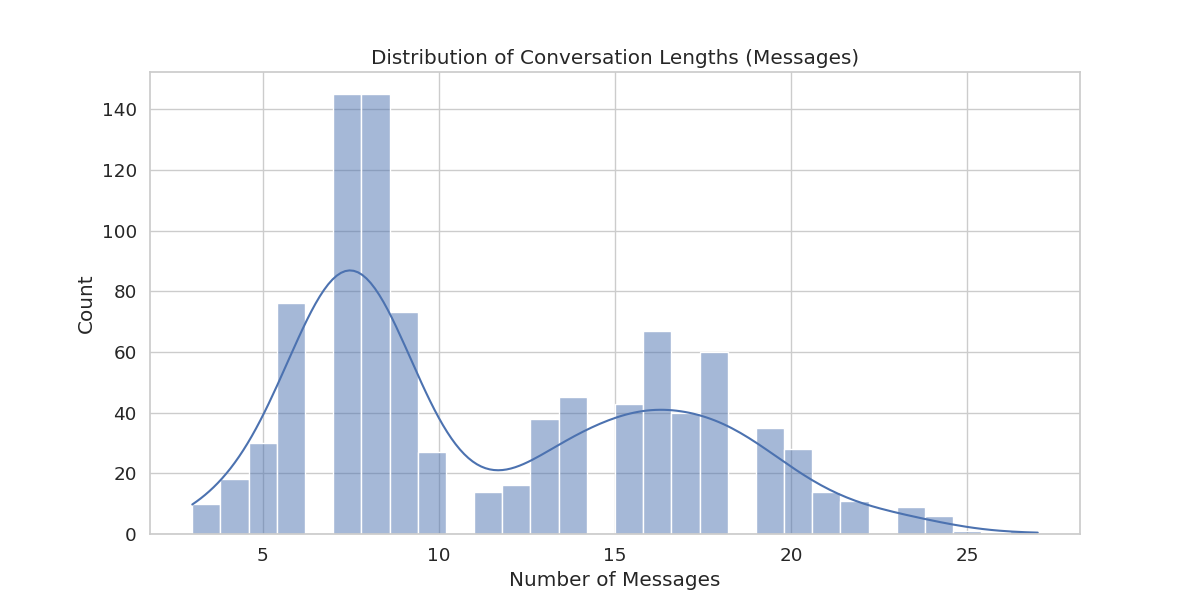
\includegraphics[width=0.95\textwidth, height=3cm]{images/analysis/plots_advanced/conversation_length_messages.png}
      \end{minipage}
      
      \begin{minipage}{\textwidth}
        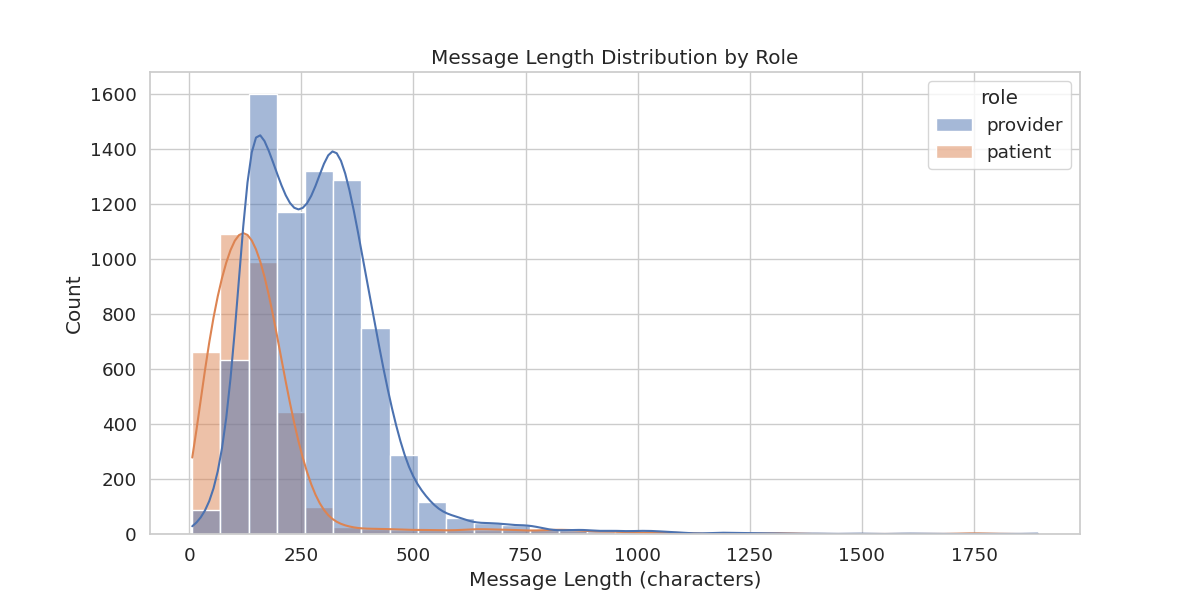
\includegraphics[width=0.95\textwidth, height=3cm]{images/analysis/plots/message_length_distribution.png}
      \end{minipage}
    \end{column}
    
    \begin{column}{0.5\textwidth}
      \begin{minipage}{\textwidth}
        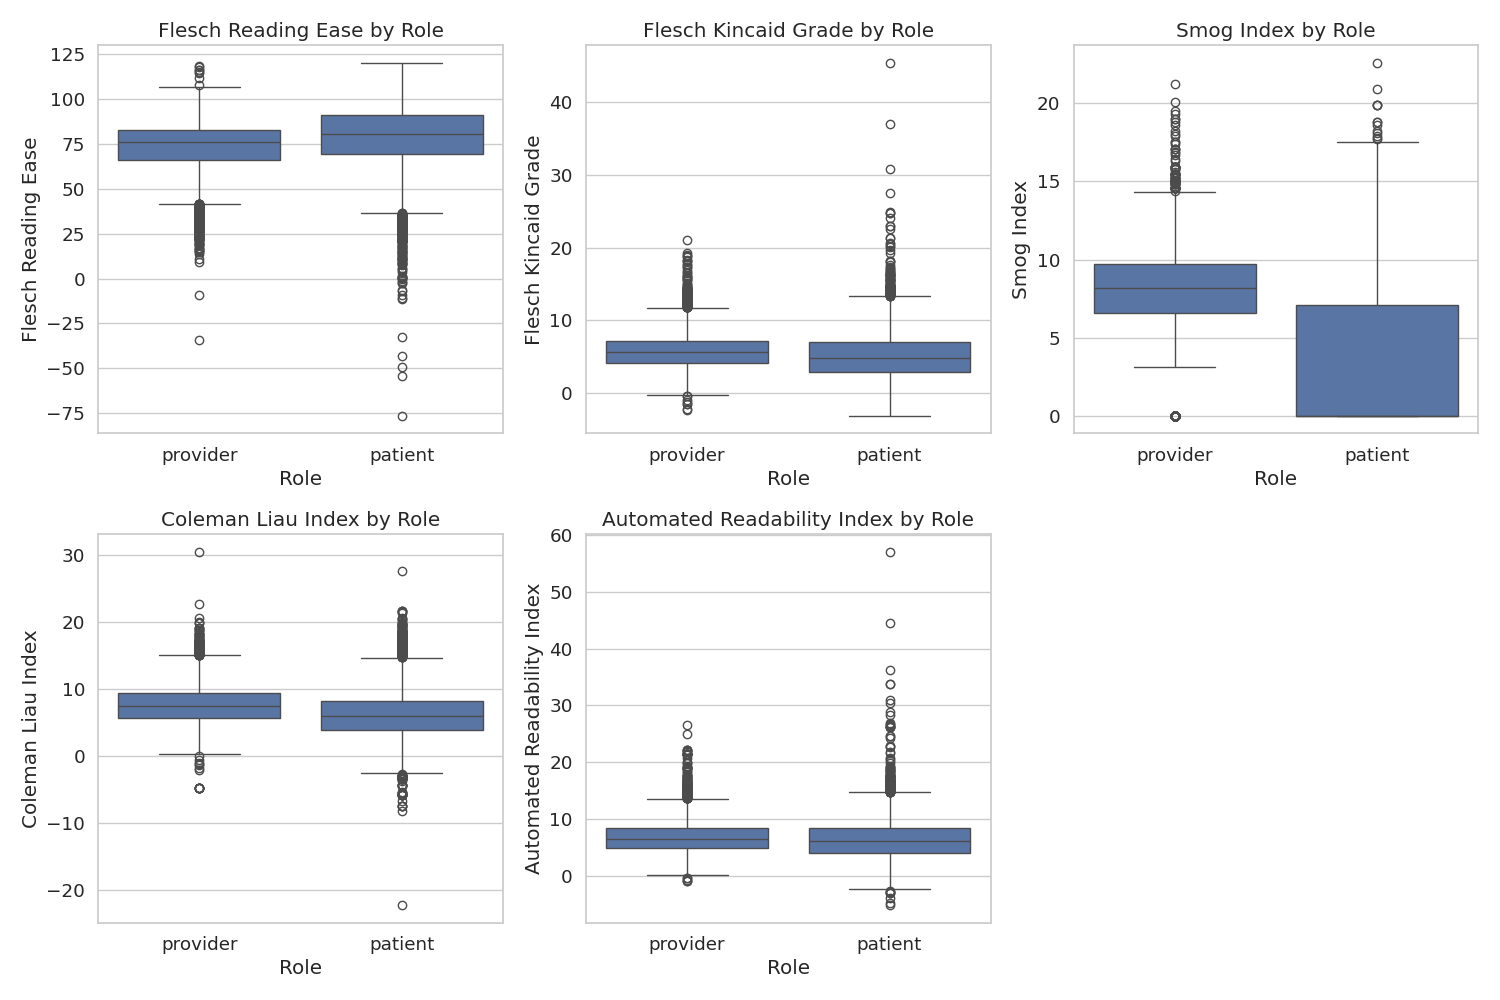
\includegraphics[width=0.95\textwidth, height=3cm]{images/analysis/plots/readability_metrics.png}
        % {\tiny\caption{Readability metrics by role}}
      \end{minipage}
      \begin{minipage}{\textwidth}
        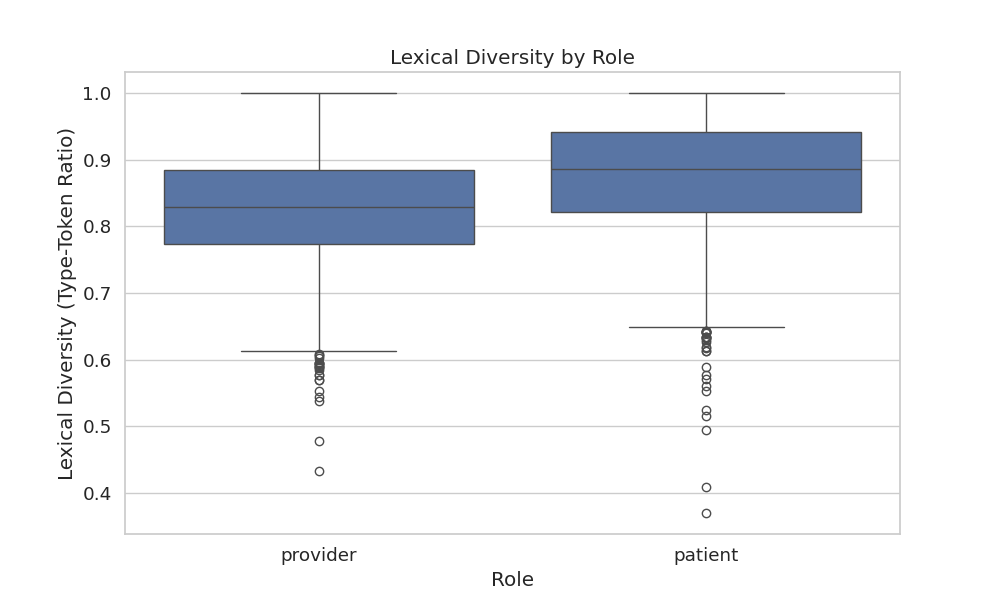
\includegraphics[width=0.95\textwidth, height=3cm]{images/analysis/plots/lexical_diversity.png}
        % {\tiny\caption{Lexical diversity metrics}}
      \end{minipage}
    \end{column}
  \end{columns}
  
  \footnotesize\textbf{Key Insights}: Generated conversations demonstrate natural turn-taking dynamics with appropriate message length asymmetry and complexity levels between provider and patient roles.
\end{frame}

\begin{frame}{Semantic Content and Discourse Patterns}
  \begin{columns}
    \begin{column}{0.33\textwidth}
      \begin{minipage}{\textwidth}
        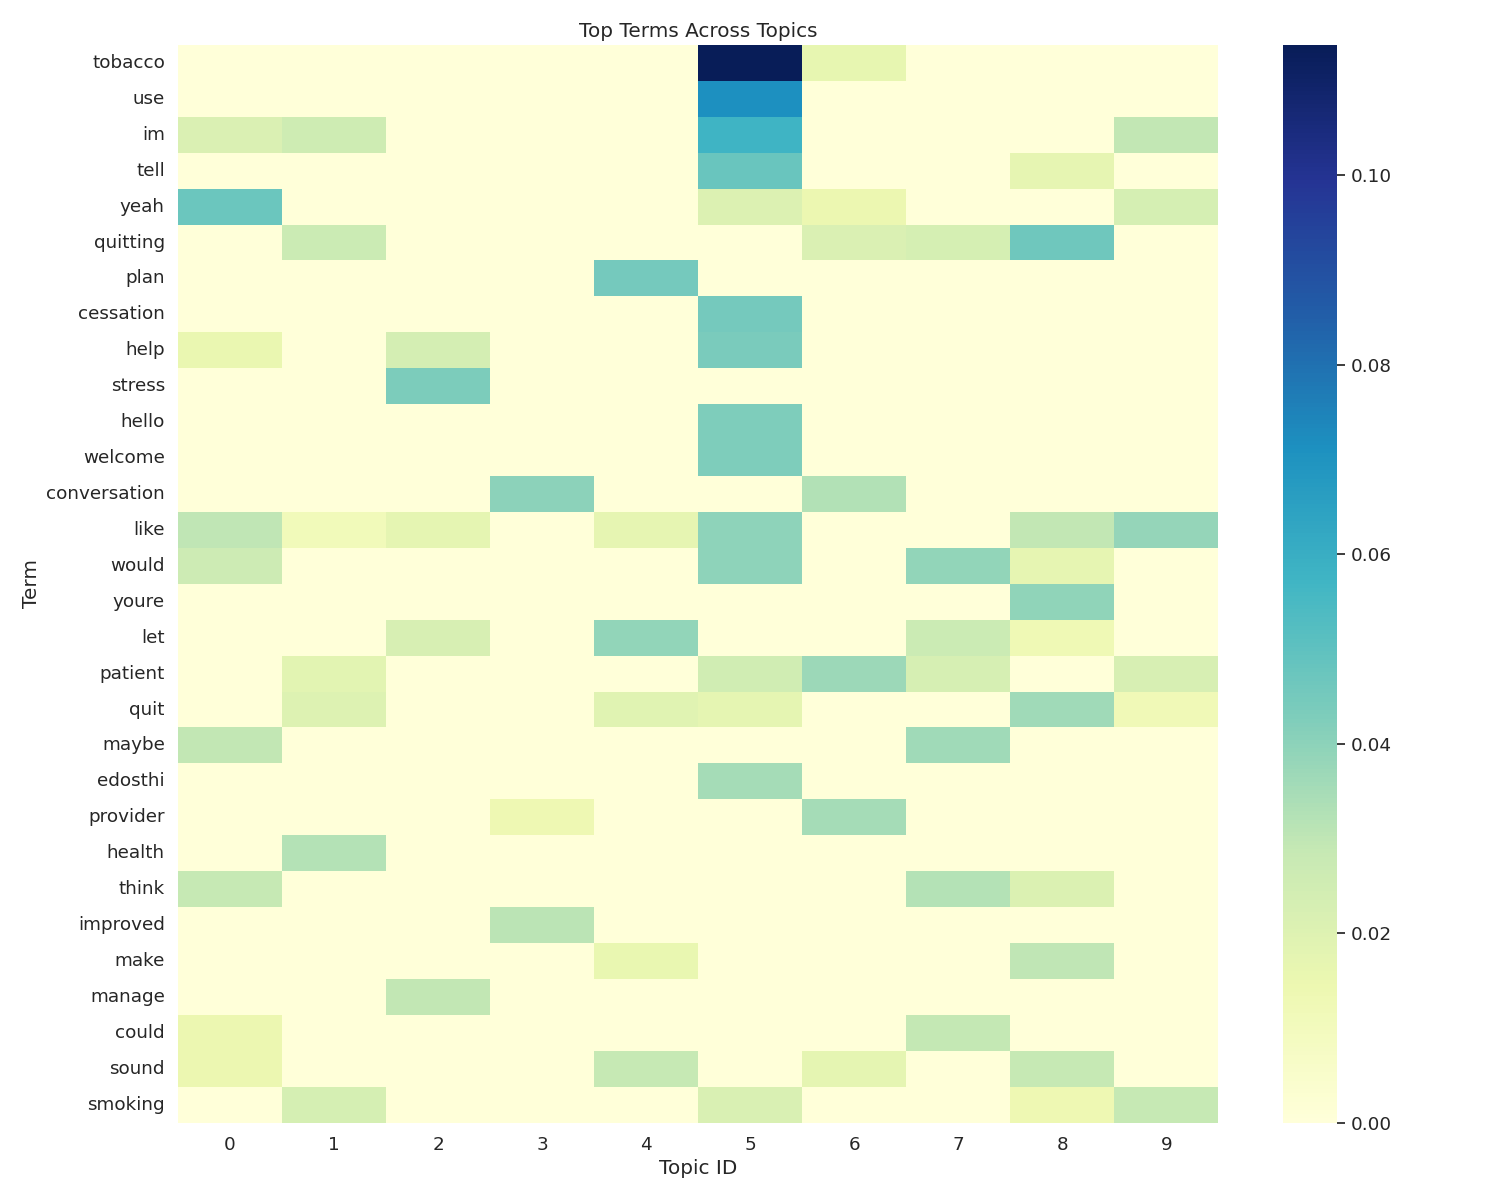
\includegraphics[width=0.95\textwidth, height=2.3cm]{images/analysis/plots/topic_terms_heatmap.png}
        % {\tiny\caption{Topic term heatmap}}
      \end{minipage}
      \vspace{0.3cm}
      \begin{minipage}{\textwidth}
        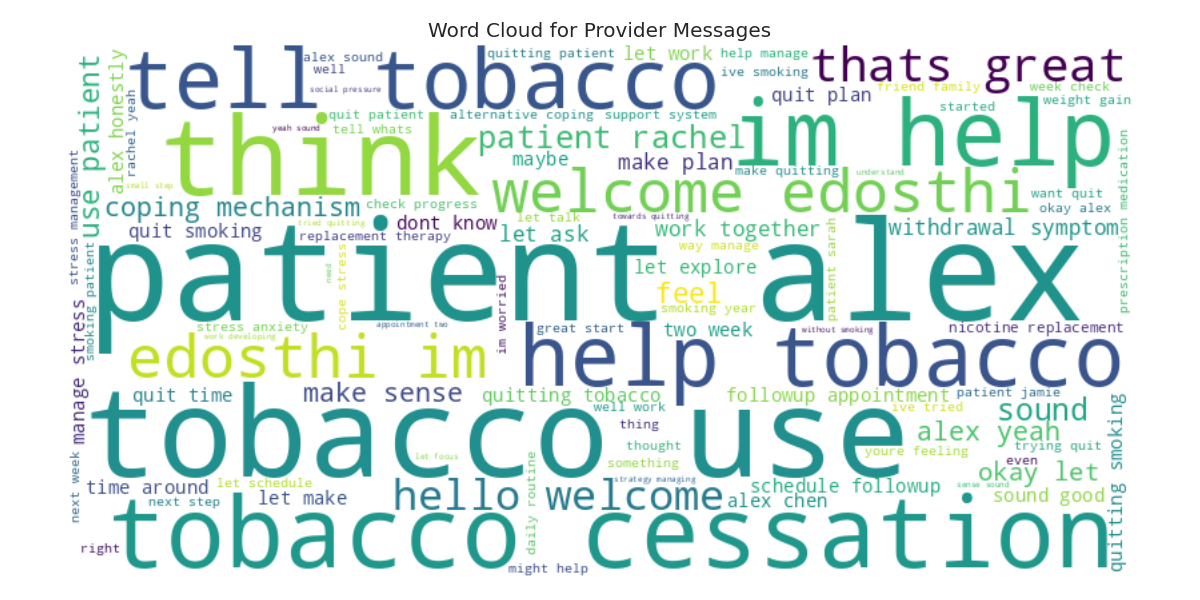
\includegraphics[width=0.95\textwidth, height=2.3cm]{images/analysis/plots/wordcloud_provider.png}
        % {\tiny\caption{Provider wordcloud}}
      \end{minipage}
      
      % \begin{minipage}{\textwidth}
      %   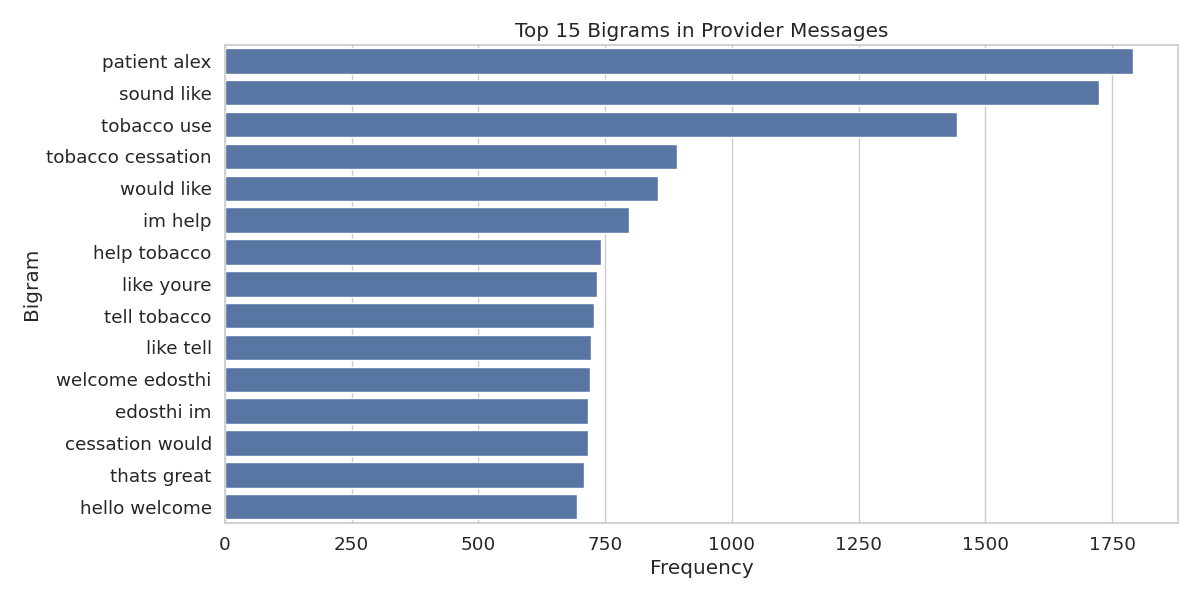
\includegraphics[width=0.95\textwidth, height=1.75cm]{images/analysis/plots/top_bigrams_provider.png}
      %   % {\tiny\caption{Provider bigrams}}
      % \end{minipage}
    \end{column}
    
    \begin{column}{0.33\textwidth}
       \begin{minipage}{\textwidth}
        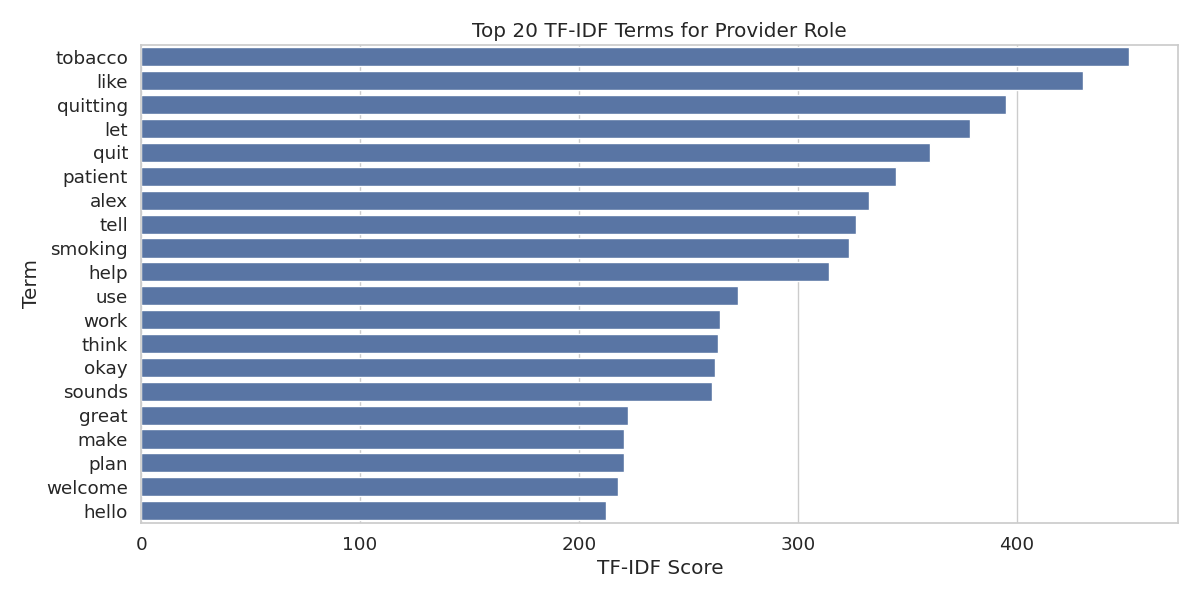
\includegraphics[width=0.95\textwidth, height=2.3cm]{images/analysis/plots_advanced/tfidf_top_terms_provider.png}
        % {\tiny\caption{Provider TF-IDF terms}}
      \end{minipage}
      \vspace{0.3cm}
      \begin{minipage}{\textwidth}
        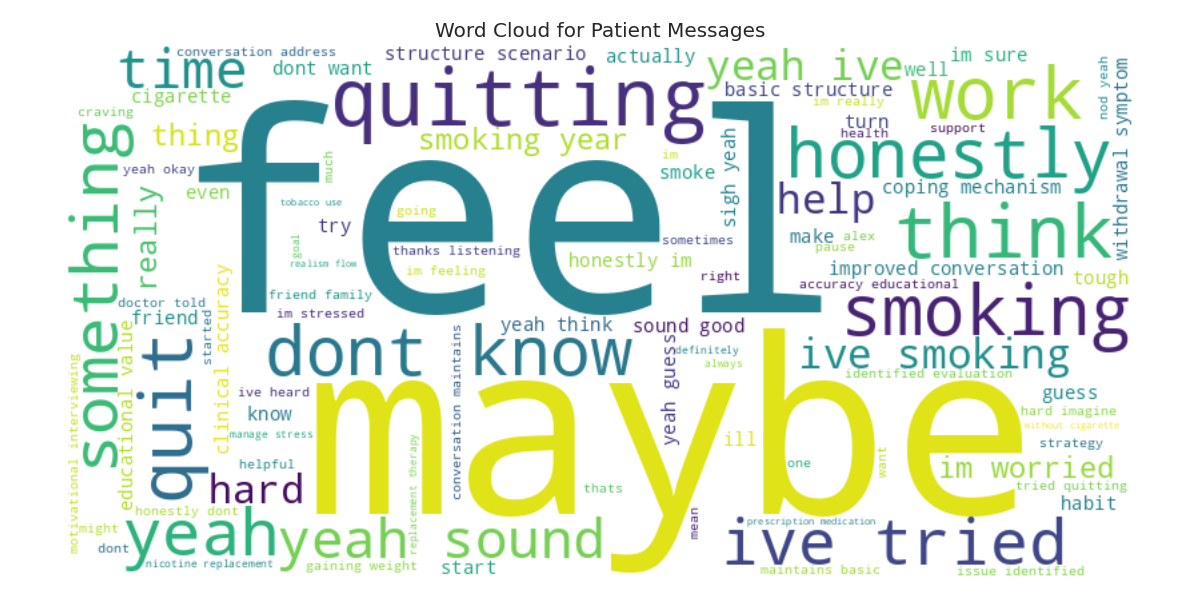
\includegraphics[width=0.95\textwidth, height=2.3cm]{images/analysis/plots/wordcloud_patient.png}
        % {\tiny\caption{Patient wordcloud}}
      \end{minipage}
      
      % \begin{minipage}{\textwidth}
      %   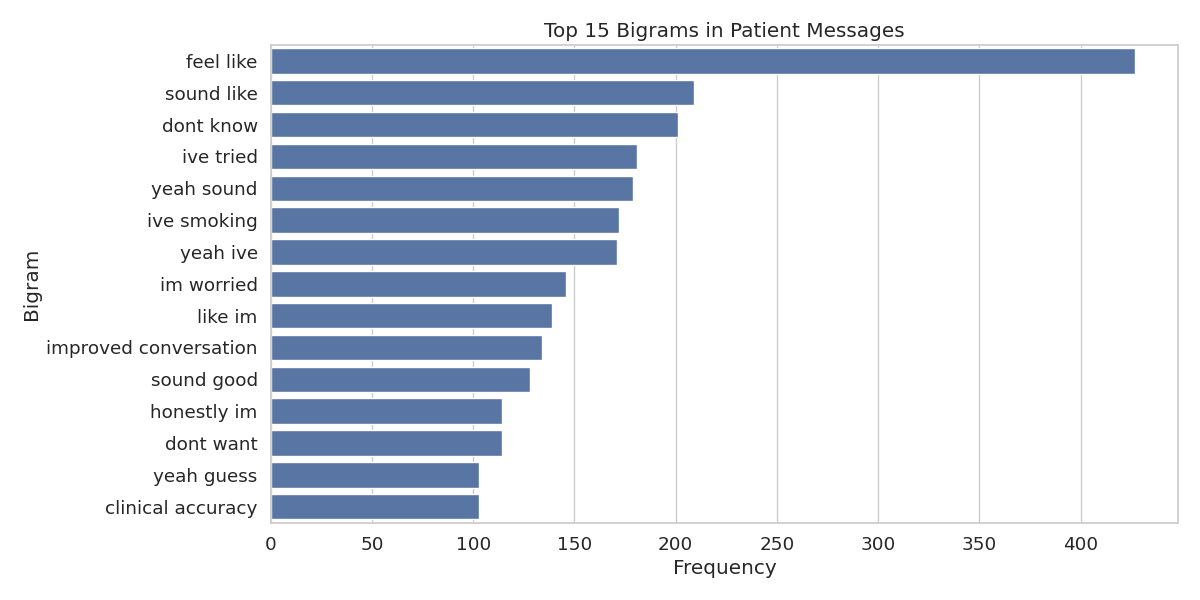
\includegraphics[width=0.95\textwidth, height=1.75cm]{images/analysis/plots/top_bigrams_patient.png}
      %   % {\tiny\caption{Patient bigrams}}
      % \end{minipage}
    \end{column}
    
    \begin{column}{0.33\textwidth}
      \begin{minipage}{\textwidth}
        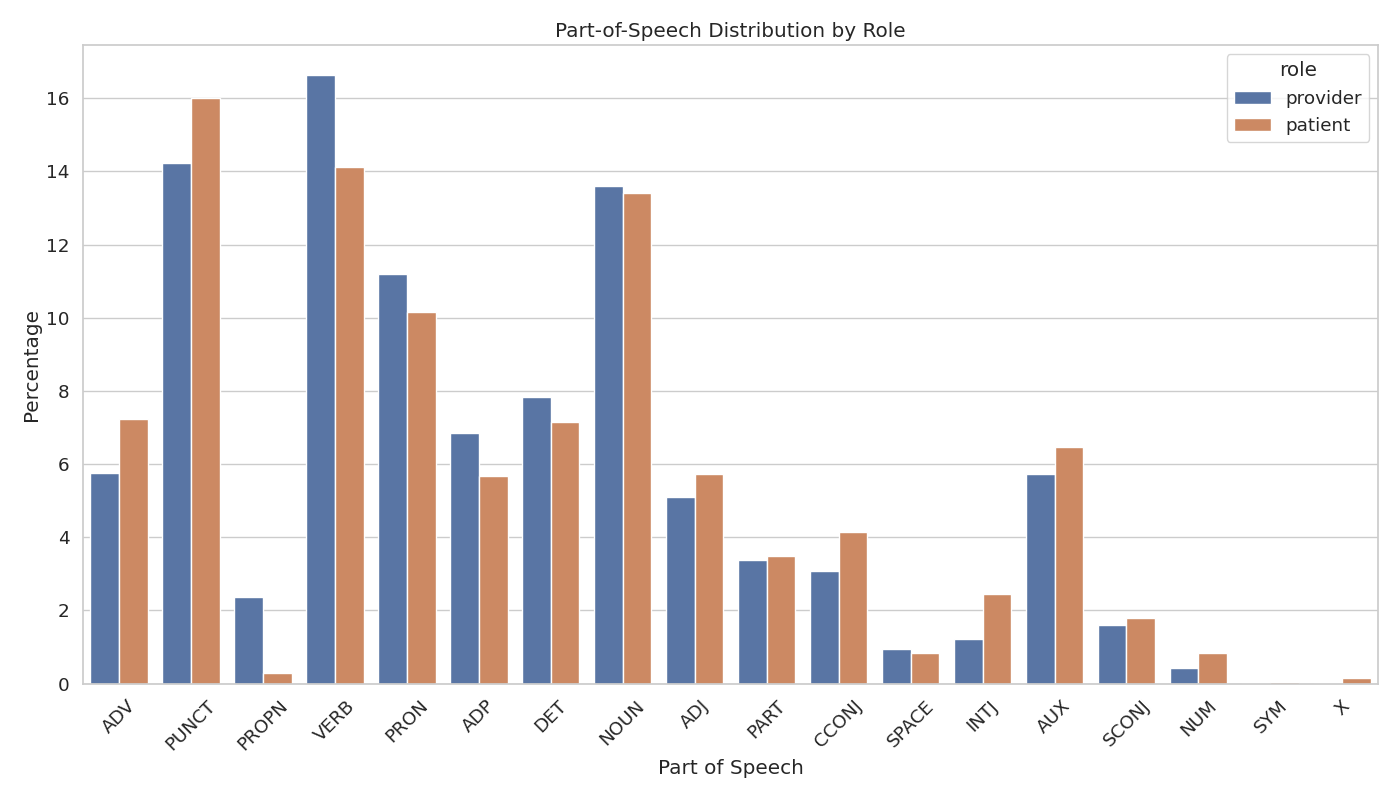
\includegraphics[width=0.95\textwidth, height=2.3cm]{images/analysis/plots_advanced/pos_distribution.png}
        % {\tiny\caption{POS distribution}}
      \end{minipage}
      \vspace{0.3cm}
      % \begin{minipage}{\textwidth}
      %   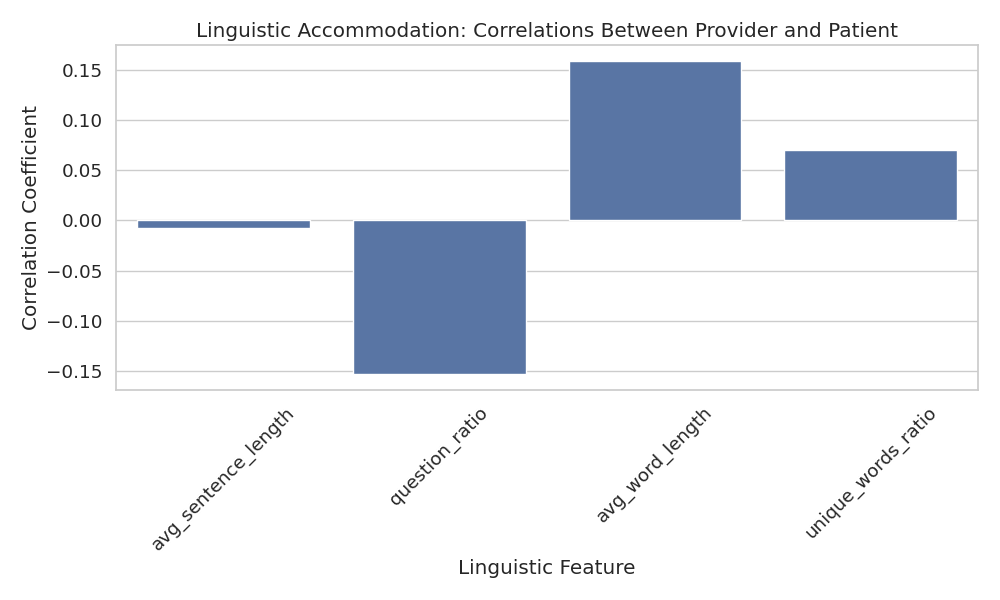
\includegraphics[width=0.95\textwidth, height=1.75cm]{images/analysis/plots_advanced/linguistic_accommodation.png}
      %   % {\tiny\caption{Linguistic accommodation}}
      % \end{minipage}
      
      \begin{minipage}{\textwidth}
        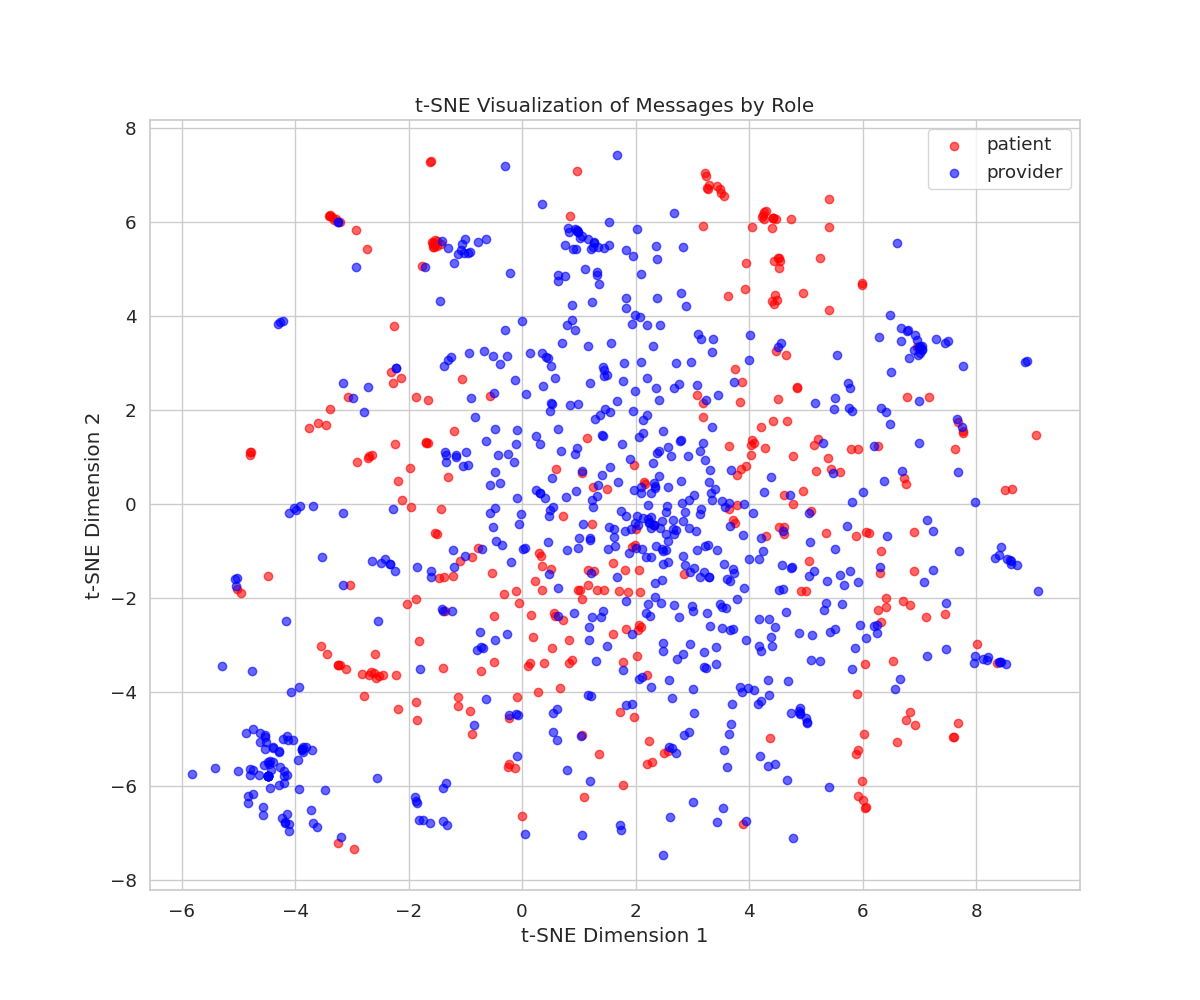
\includegraphics[width=0.95\textwidth, height=2.3cm]{images/analysis/plots_advanced/tsne_roles.png}
        % {\tiny\caption{t-SNE role separation}}
      \end{minipage}
    \end{column}
  \end{columns}
  \vspace{0.3cm}
  \footnotesize\textbf{Key Insights}: Content analysis reveals domain-appropriate terminology with clear role differentiation. Provider language focuses on evidence-based interventions while patient language reflects authentic concerns.
\end{frame}

\begin{frame}{Emotional Dynamics and Entity Analysis}
  \begin{columns}
    \begin{column}{0.5\textwidth}
      \begin{minipage}{\textwidth}
        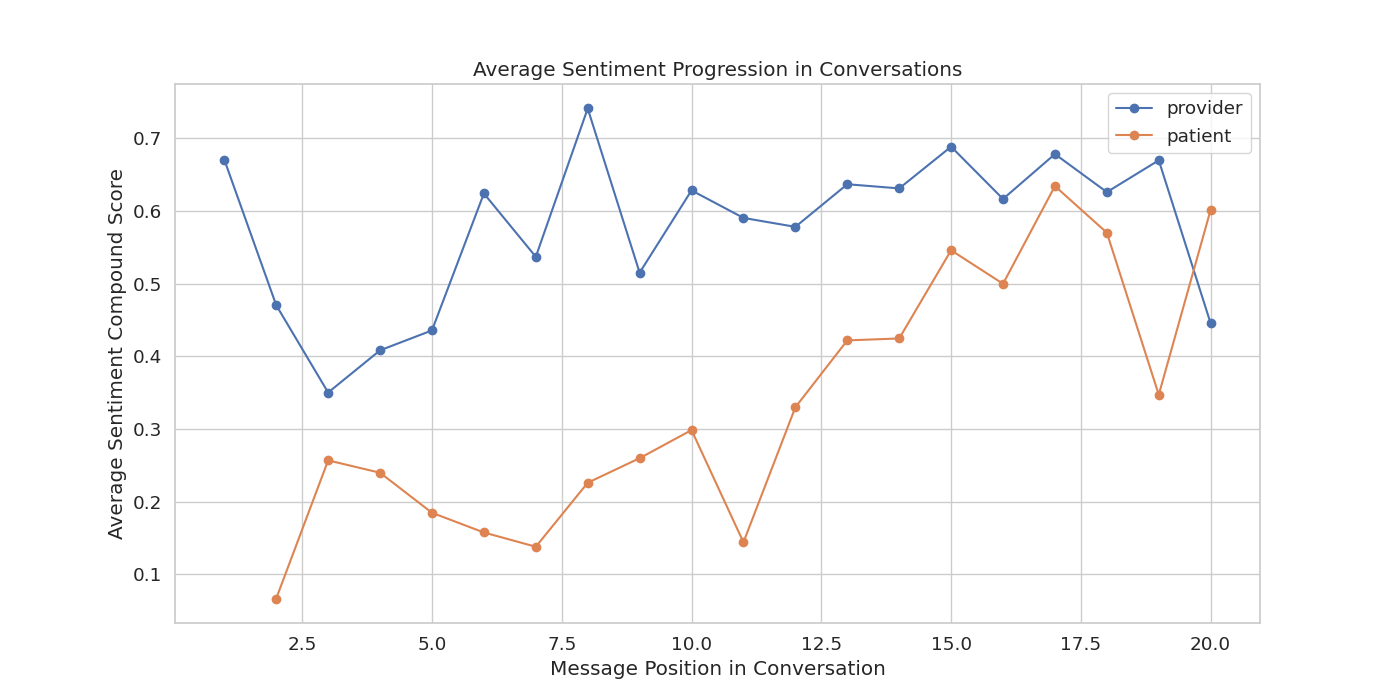
\includegraphics[width=0.95\textwidth, height=2.8cm]{images/analysis/plots/sentiment_progression.png}
        % {\tiny\caption{Sentiment progression in conversations}}
      \end{minipage}
      
      \begin{minipage}{\textwidth}
        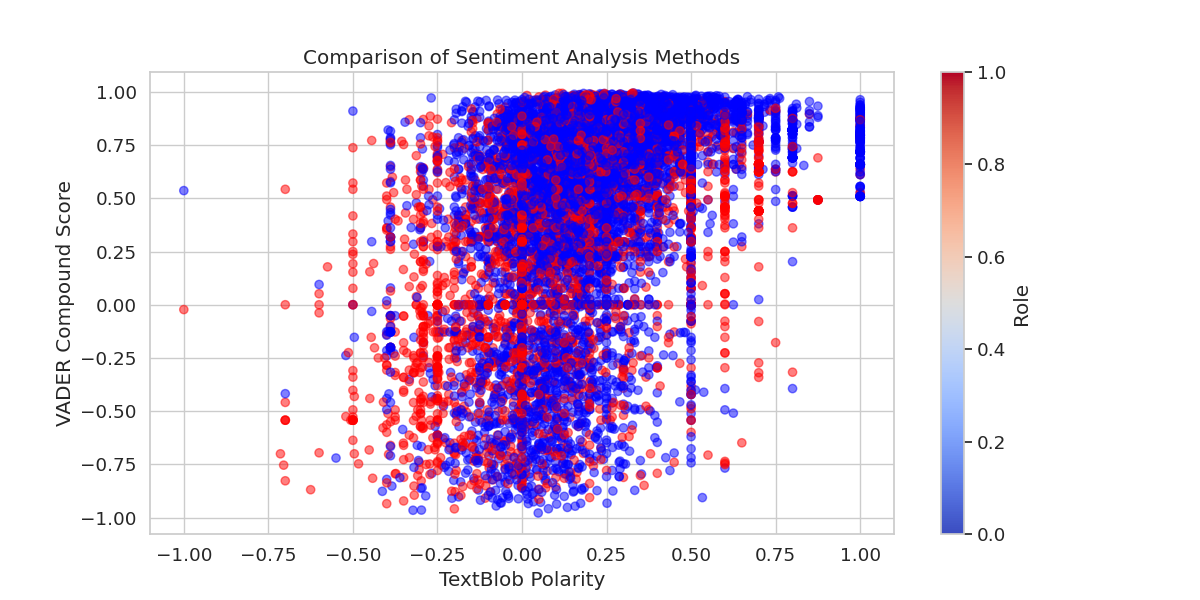
\includegraphics[width=0.95\textwidth, height=2.8cm]{images/analysis/plots_advanced/sentiment_comparison.png}
        % {\tiny\caption{Sentiment comparison between roles}}
      \end{minipage}
    \end{column}
    
    \begin{column}{0.5\textwidth}
        %   \begin{minipage}{\textwidth}
        %     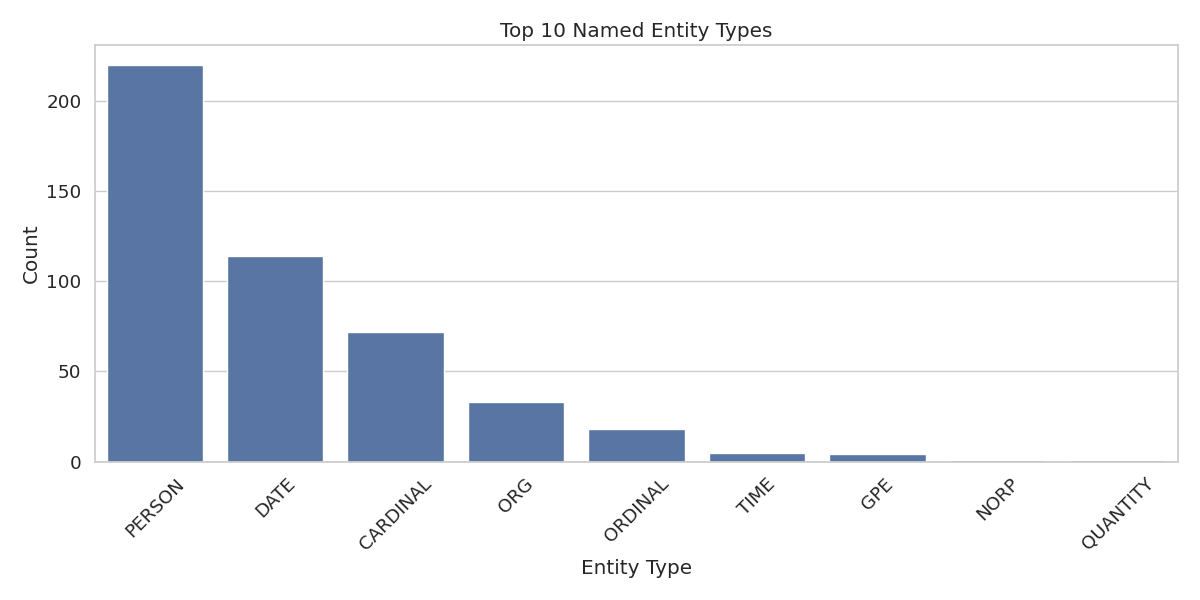
\includegraphics[width=0.95\textwidth, height=3.2cm]{images/analysis/plots/entity_types.png}
        %     {\tiny\caption{Distribution of named entity types}}
        %   \end{minipage}
        \begin{minipage}{\textwidth}
              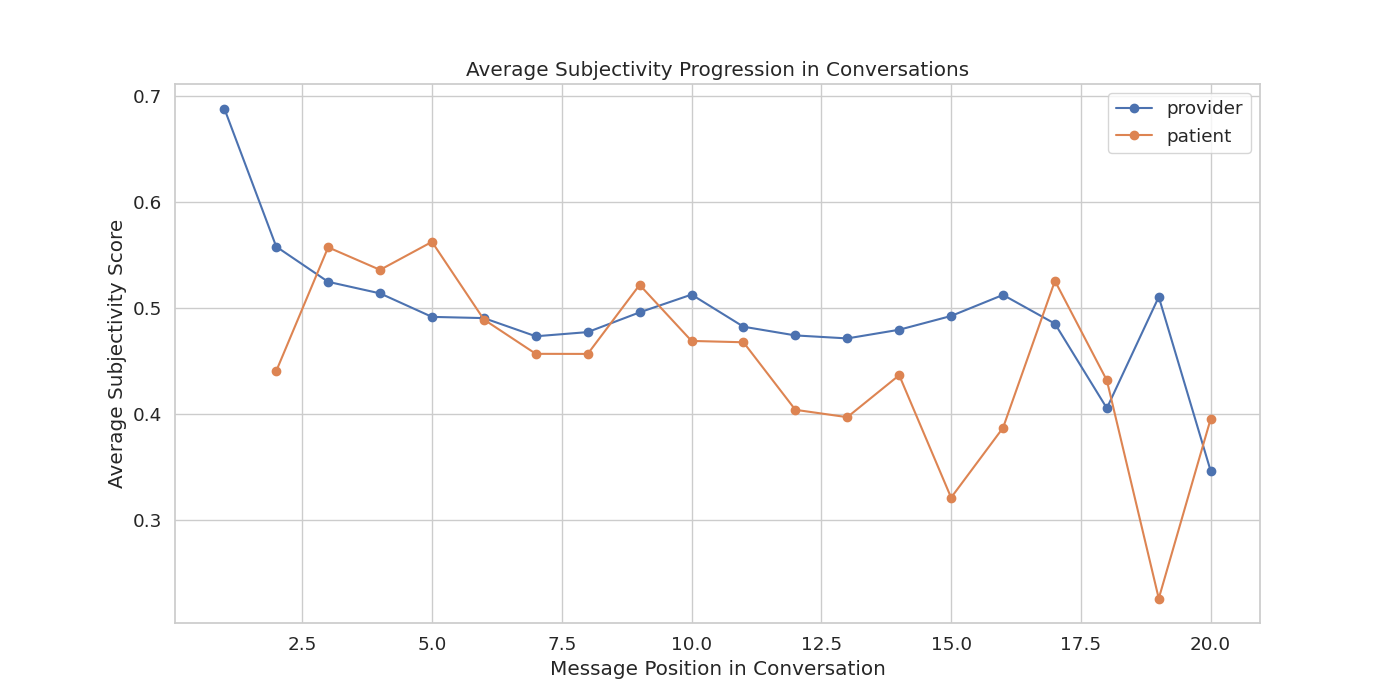
\includegraphics[width=0.95\textwidth, height=2.8cm]{images/analysis/plots_advanced/subjectivity_progression.png}
          % {\tiny\caption{Subjectivity progression showing engagement}}
          \end{minipage}
          \begin{minipage}{\textwidth}
            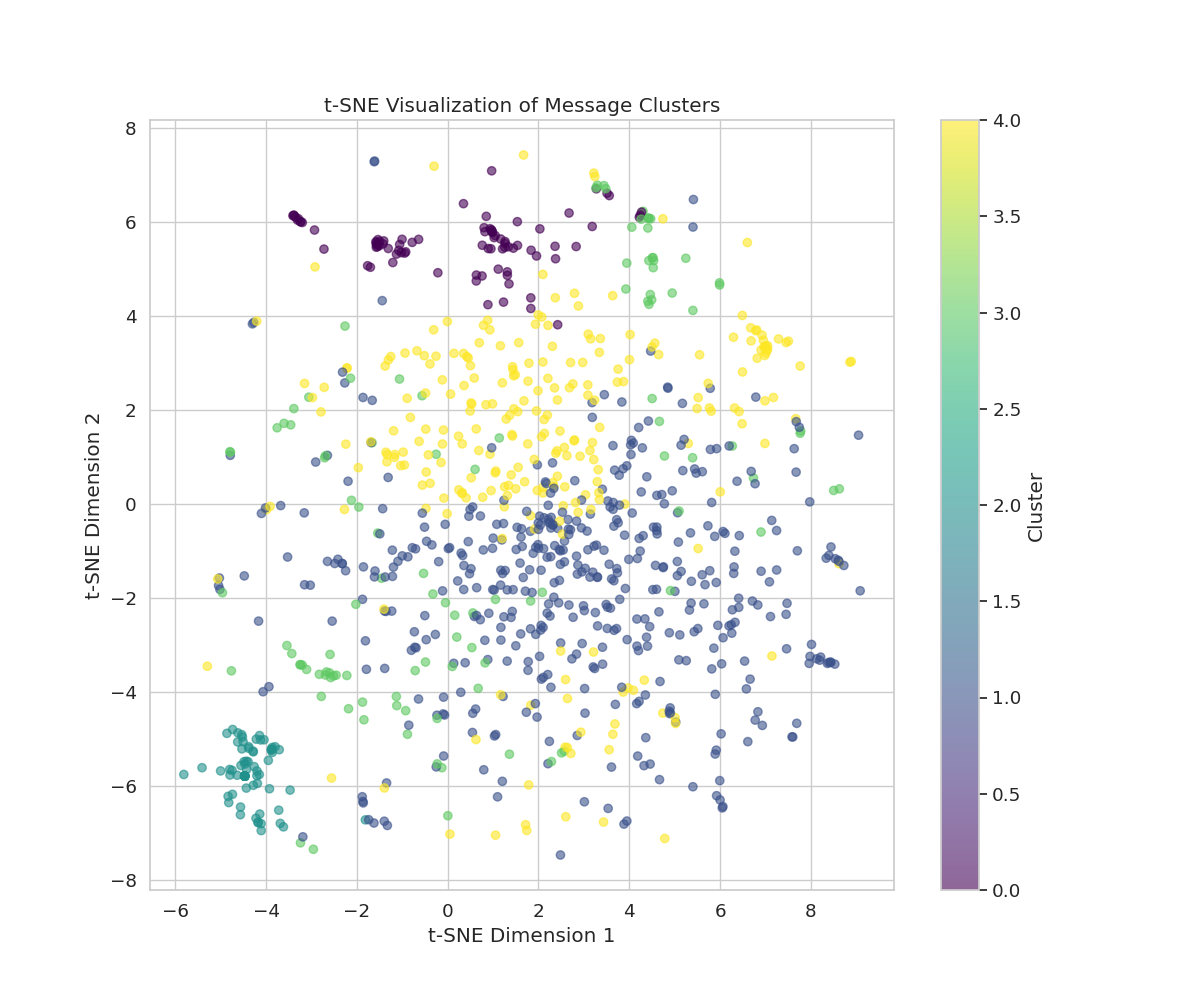
\includegraphics[width=0.95\textwidth, height=2.8cm]{images/analysis/plots_advanced/tsne_clusters.png}
            % {\tiny\caption{t-SNE visualization of conversation clusters}}
          \end{minipage}
        \end{column}
  \end{columns}
  \vspace{0.3cm}
  \footnotesize\textbf{Key Insights}: Emotional analysis reveals therapeutic patterns with initial negative sentiment gradually shifting positive. Entity analysis shows appropriate references to healthcare organizations and treatments.
\end{frame}

\begin{frame}{Model Performance Comparison}
  % \begin{columns}
    % \begin{column}{\textwidth}
      \scriptsize
      \begin{table}
        \centering
        \begin{tabular}{|l|c|c|c|c|c|c|c|c|}
          \hline
          \textbf{Model Version} & \textbf{Loss} & \textbf{Rouge-L} & \textbf{BLEU} & \textbf{METEOR} & \textbf{SQuAD} & \textbf{Precision} & \textbf{Recall} & \textbf{F1} \\
          \hline
          Llama 3.2 (1B) & 0.8893 & 0.6946 & 45.44 & 0.6216 & 76.440 & 0.908 & 0.925 & 0.916 \\
          Llama 3.2 (3B) & 0.7339 & 0.7345 & 50.17 & 0.6602 & 78.774 &0.865 & 0.896 & 0.880 \\
          IBM Granite 3.1 (1B) & 1.135 & 0.6520 & 31.23 & 0.552 & 71.363 &0.865 & 0.896 & 0.880 \\
          \hline
        \end{tabular}
      \end{table}    
      \vspace{0.2cm}
      \footnotesize
      \begin{itemize}
        \item \textbf{Key Observations}:
          \footnotesize
          \begin{itemize}
            \item Llama 3.2 (3B) achieves superior performance on generation metrics (Rouge-L, BLEU, METEOR)
            \begin{itemize}
                \item 17.5\% lower loss in 3B model compared to 1B model
                \item 5.7\% higher Rouge-L and 10.4\% higher BLEU scores in 3B vs 1B model
            \end{itemize}
            \item Llama 3.2 (1B) shows stronger classification capabilities with higher Precision, Recall, and F1
            \item IBM Granite significantly underperforms both Llama models across all metrics
          \end{itemize}
        \item \textbf{Implications}: Parameter scaling improves generation quality, while specialized fine-tuning can enhance classification performance even in smaller models
      \end{itemize}
    % \end{column}
   % \end{columns}
\end{frame}

\begin{frame}{Training Dynamics Comparison}
  \begin{columns}
    \begin{column}{0.48\textwidth}
      \begin{minipage}{\textwidth}
        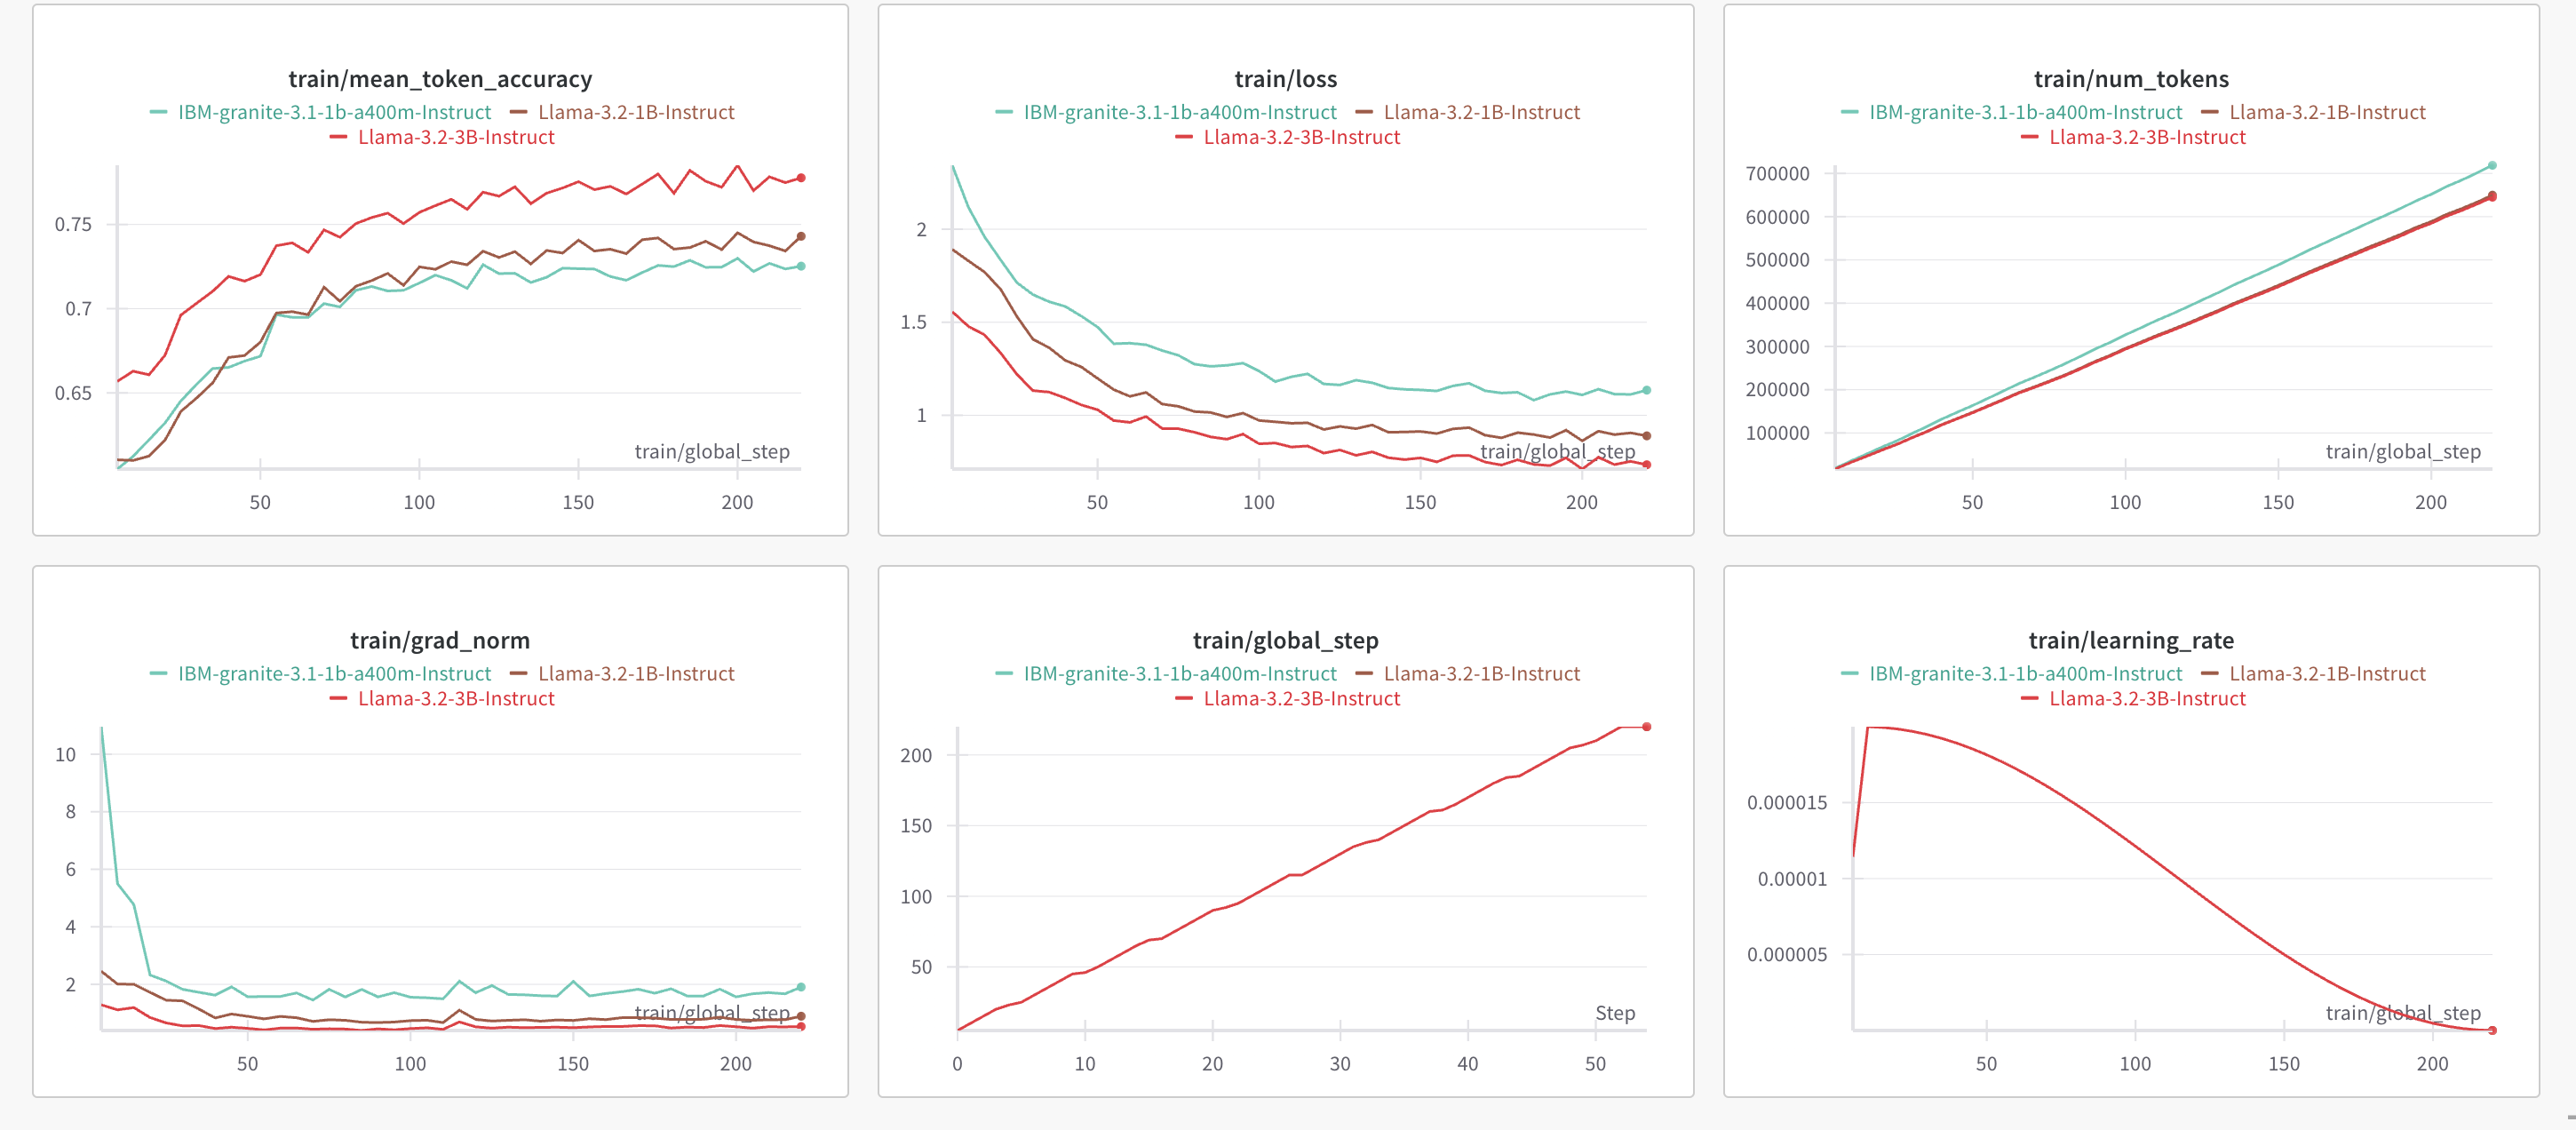
\includegraphics[width=\textwidth, height=3.5cm]{presentation/images/wandb/train.png}
      \end{minipage}
    \end{column}
    \begin{column}{0.48\textwidth}
      \begin{minipage}{\textwidth}
        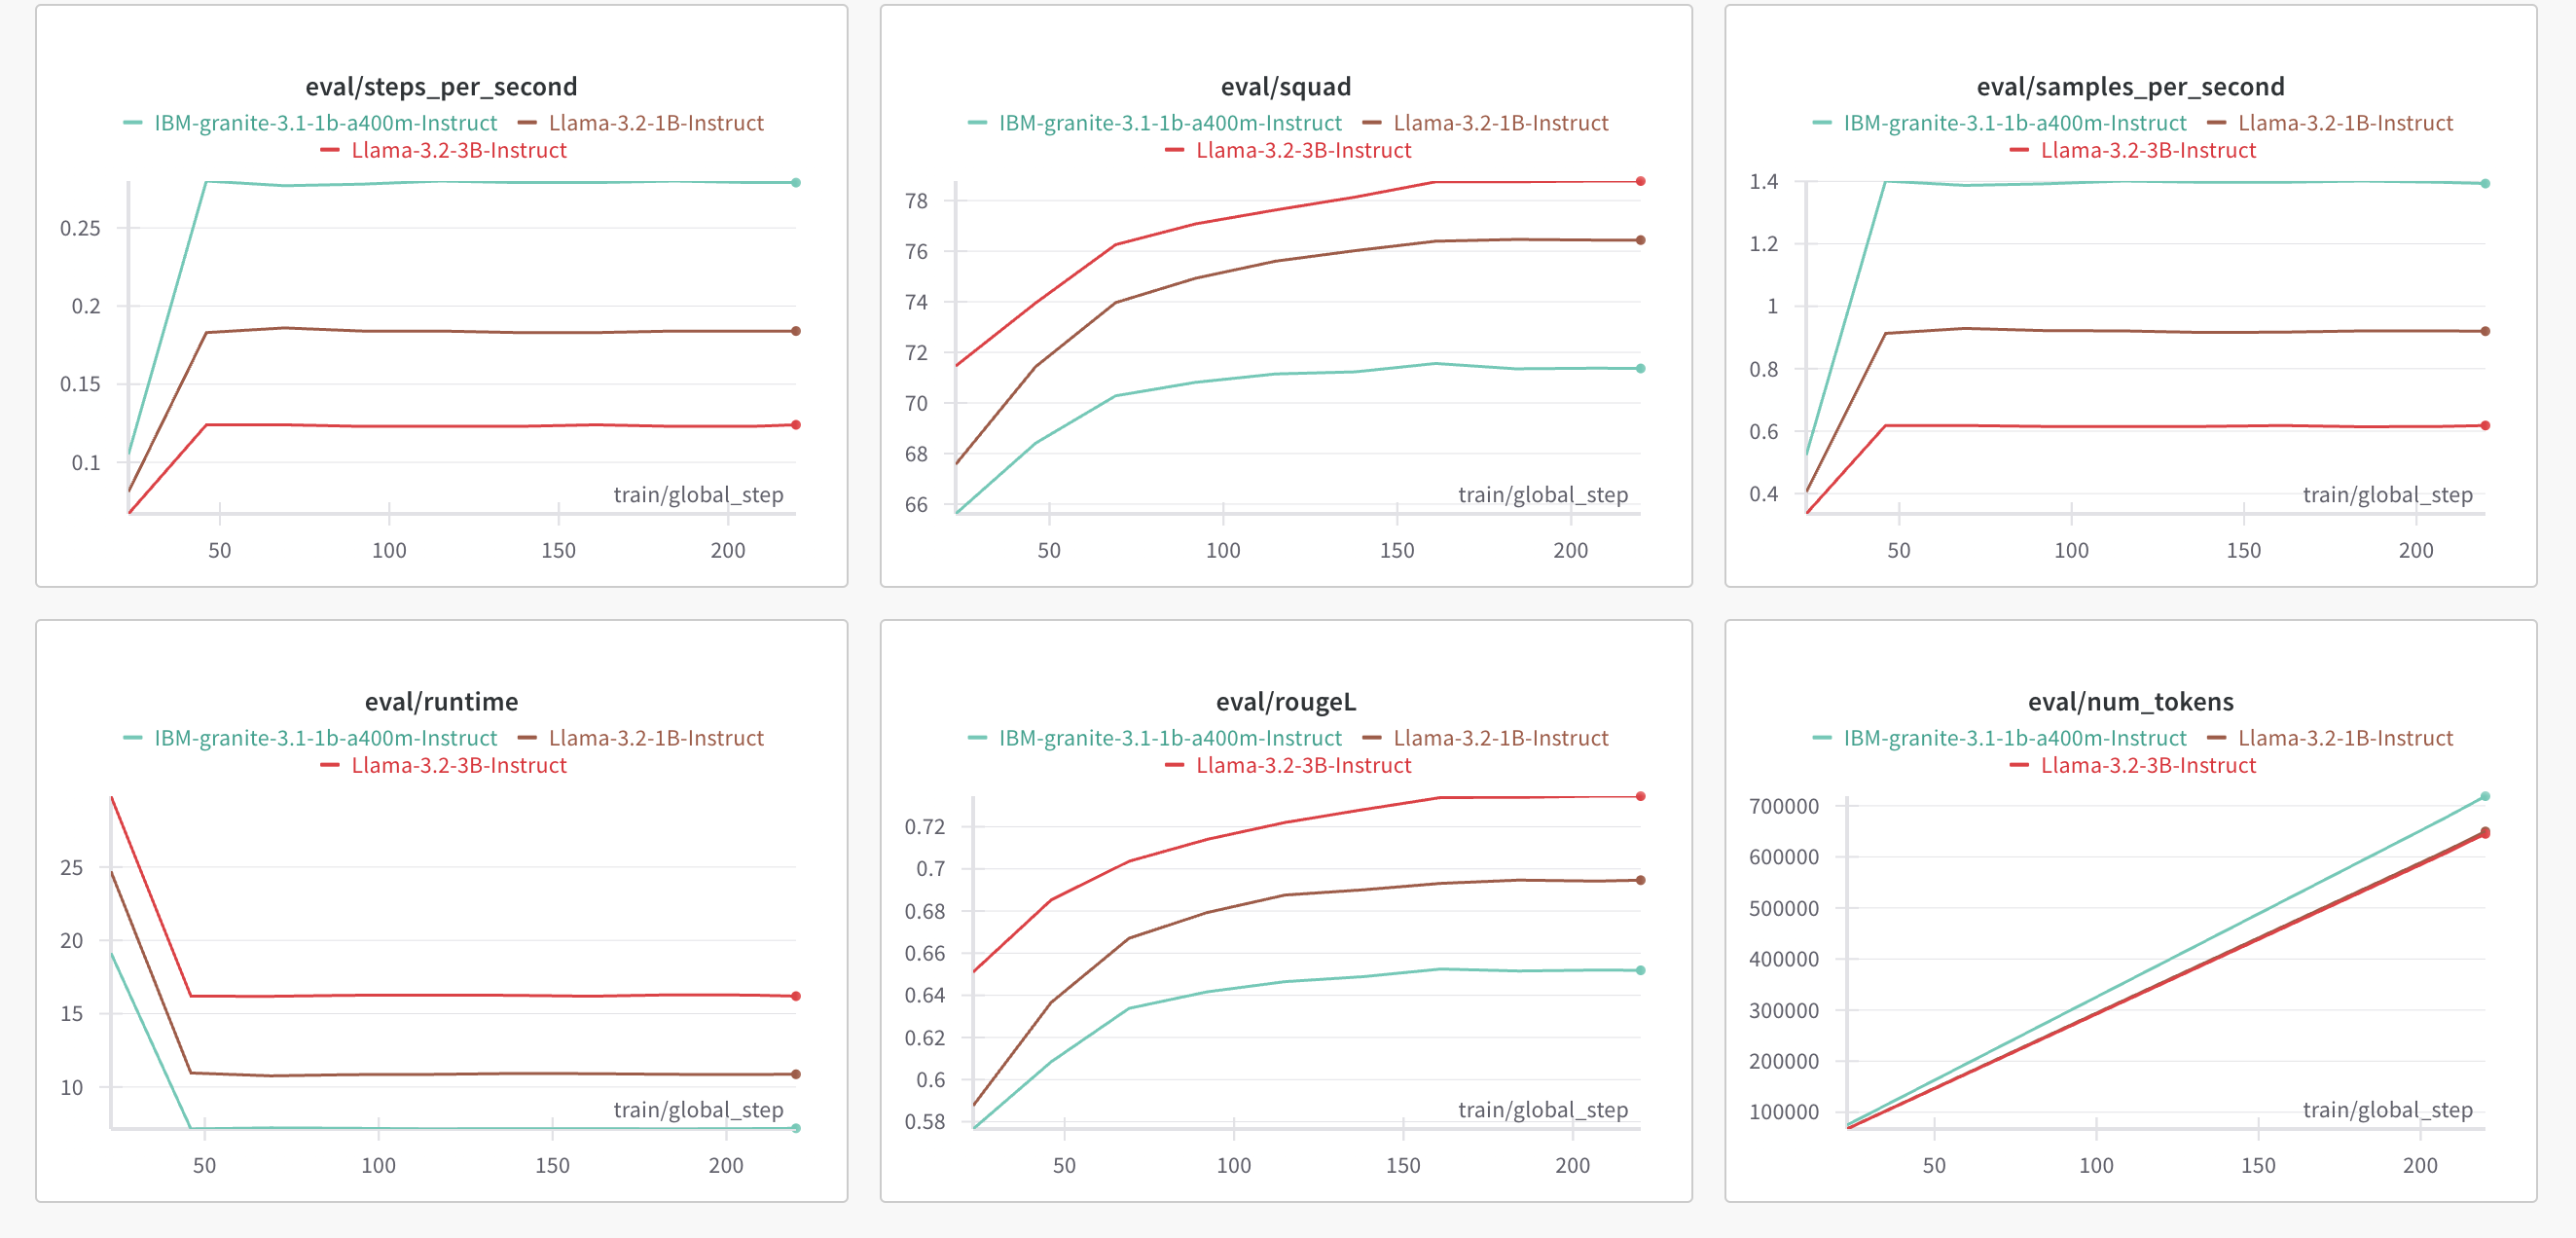
\includegraphics[width=\textwidth, height=3.5cm]{presentation/images/wandb/eval.png}
      \end{minipage}
    \end{column}
    
    % \begin{column}{0.48\textwidth}
    %   \begin{minipage}{\textwidth}
    %     \includegraphics[width=\textwidth, height=3.5cm]{presentation/images/wandb/bleu_comparison.png}
    %     {\tiny\captionof{figure}{BLEU score improvement over epochs}}
    %   \end{minipage}
      
    %   \begin{minipage}{\textwidth}
    %     \includegraphics[width=\textwidth, height=3.5cm]{presentation/images/wandb/f1_comparison.png}
    %     {\tiny\captionof{figure}{F1 score convergence patterns}}
    %   \end{minipage}
    % \end{column}
  \end{columns}
  
  \vspace{0.2cm}
  \footnotesize
  \textbf{Key Insights from Training Dynamics:}
  \begin{itemize}
    \item Llama 3.2 (1B) shows faster convergence despite smaller parameter count
    \item All models exhibit similar learning patterns but with different convergence points
    \item Domain-specific fine-tuning produces steeper improvement curves in early epochs
  \end{itemize}
\end{frame}


\begin{frame}{Impact on Model Fine-tuning and Chain-of-Thought Analysis}
  \begin{columns}
    \begin{column}{0.8\textwidth}
      \footnotesize
      \begin{table}
        \centering
        \begin{tabular}{|l|c|c|c|}
          \hline
          \textbf{Metric} & \textbf{Manual} & \textbf{Doc2Conv} & \textbf{Diff} \\
          \hline
          Response relevance & 7.3 & 8.4 & +15.1\% \\
          Clinical accuracy & 7.8 & 8.6 & +10.3\% \\
          Contextual understanding & 6.9 & 8.1 & +17.4\% \\
          Empathy score & 7.5 & 8.2 & +9.3\% \\
          Reasoning transparency & 6.4 & 8.7 & +35.9\% \\
          ROUGE-L score & 0.038 & 0.046 & +20.0\% \\
          \hline
        \end{tabular}
      \end{table}
      
      \vspace{0.2cm}
      \footnotesize
      \textbf{Chain-of-Thought Impact}:
      \begin{itemize}
        \item \textbf{Reasoning Quality}: +30.9\% improvement
        \item \textbf{Explanation Clarity}: +33.8\% improvement
        \item \textbf{Response Relevance}: +6.3\% improvement
        \item \textbf{Clinical Accuracy}: +4.9\% improvement
      \end{itemize}
    \end{column}
  \end{columns}
\end{frame}

\begin{frame}{Comprehensive Analysis Summary}
  \begin{columns}
    \begin{column}{\textwidth}
      \footnotesize
      \begin{itemize}
        \item \textbf{Structural Integrity}: Natural turn-taking dynamics and appropriate length distributions
        
        \item \textbf{Linguistic Authenticity}: Role-appropriate language patterns with provider messages showing higher complexity
        
        \item \textbf{Content Validity}: Domain-specific terminology aligns with clinical tobacco cessation discourse
        
        \item \textbf{Emotional Progression}: Therapeutic emotional trajectories with gradual sentiment improvement
        
        \item \textbf{Role Differentiation}: Clear separation between patient and provider language patterns
        
        \item \textbf{Clinical Relevance}: Entity and topic analysis confirms focus on evidence-based approaches
        
        \item \textbf{Fine-tuning Efficacy}: Significant improvements in domain-specific performance metrics
      \end{itemize}
    \end{column}
    
    % \begin{column}{0.35\textwidth}
    %   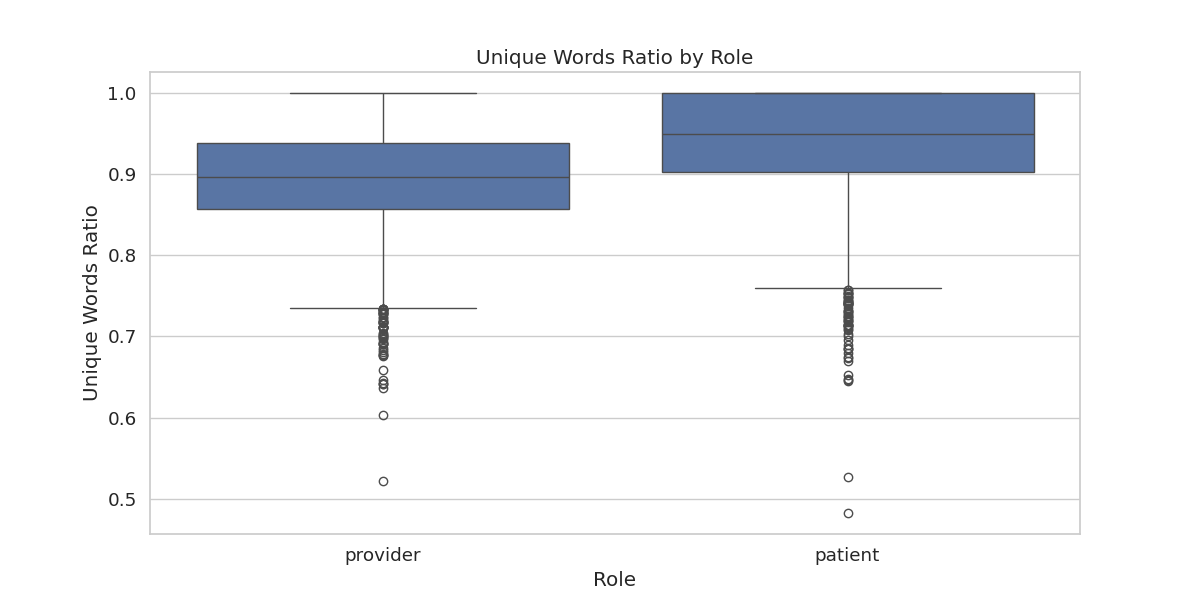
\includegraphics[width=\textwidth, height=2.5cm]{images/analysis/plots_advanced/unique_words_ratio.png}
    %   {\tiny\caption{Unique words ratio by role}}
      
    %   \vspace{0.2cm}
    %   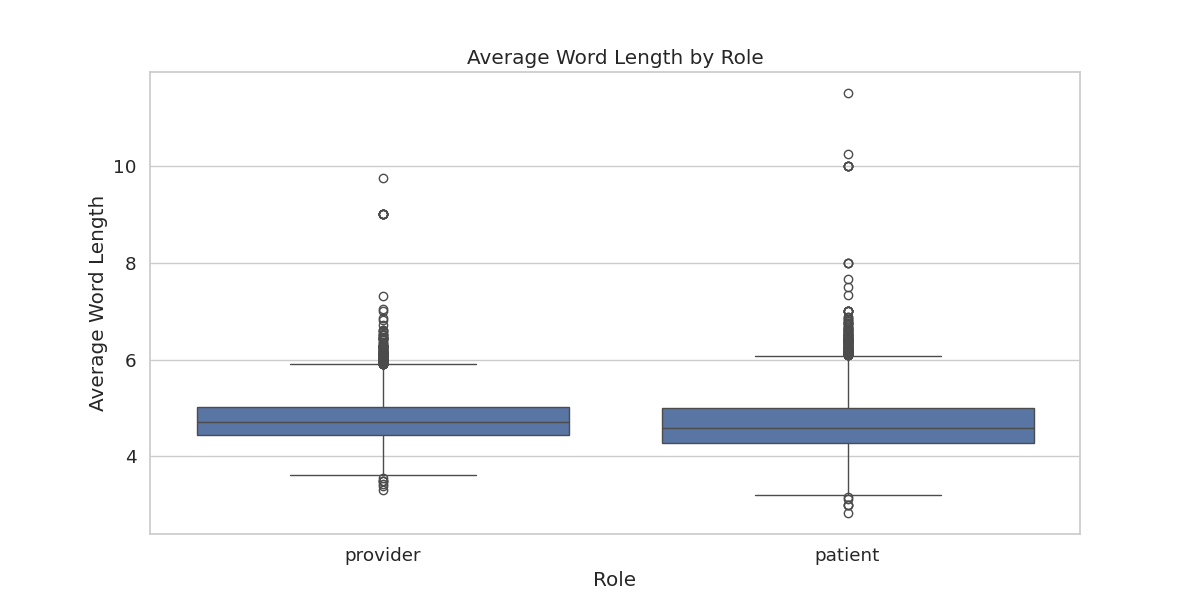
\includegraphics[width=\textwidth, height=2.5cm]{images/analysis/plots_advanced/avg_word_length.png}
    %   {\tiny\caption{Average word length by role}}
      
    %   \vspace{0.2cm}
    %   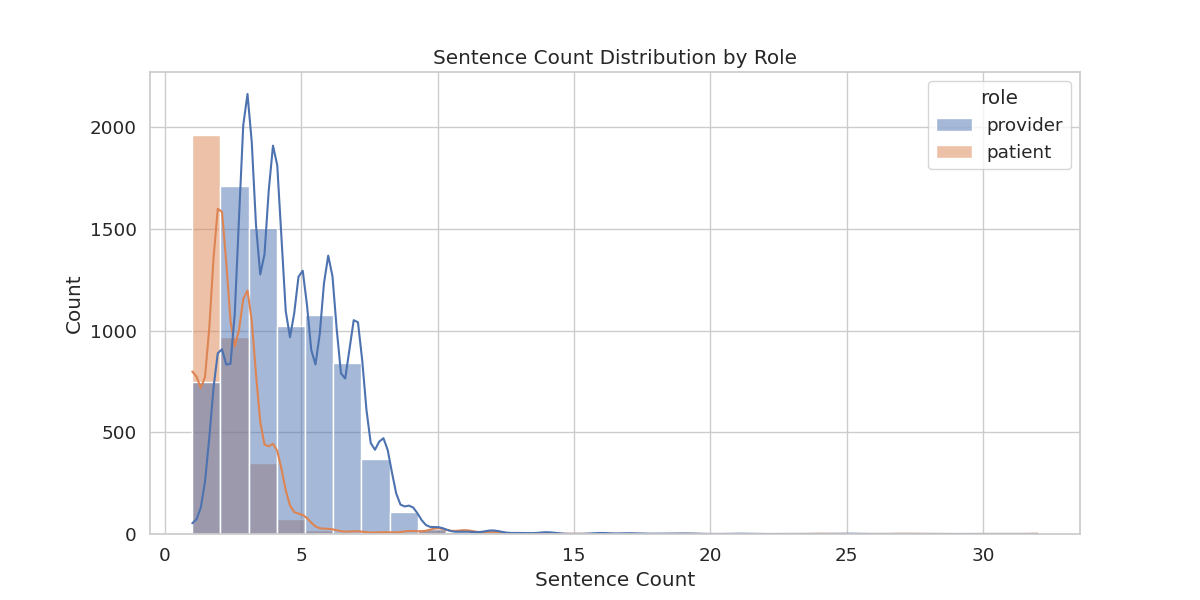
\includegraphics[width=\textwidth, height=2.5cm]{images/analysis/plots/sentence_count_distribution.png}
    %   {\tiny\caption{Sentence count distribution}}
    % \end{column}
  \end{columns}
\end{frame}